\documentclass[12pt]{article}
\usepackage{amsfonts}
\usepackage{comment}
\usepackage{tikz}
\usepackage{forest}
\usetikzlibrary{arrows,automata}
\begin{document}

\noindent
Jason Downing \\
Email: jason\_downing@student.uml.edu \\
Foundations of Computer Science \\
Homework \#3 - Chapter 1: DFA, NFA\\
10/31/2016 \\

%*********************************************************************************
% 2.1 here

\noindent
2.1 \\
Recall the CFC G4 that we gave in Example 2.4. \\

\noindent
a. \\
Parse tree for $a$: \\
\begin{center}
	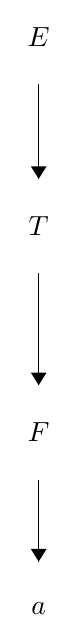
\begin{tikzpicture}[scale=0.2]
	\tikzstyle{every node}+=[inner sep=0pt]
	\draw (31.3,-11.1) node {$E$};
	\draw (31.3,-23.1) node {$T$};
	\draw (31.3,-47.4) node {$a$};
	\draw (31.3,-36.2) node {$F$};
	\draw [black] (31.3,-14.1) -- (31.3,-20.1);
	\fill [black] (31.3,-20.1) -- (31.8,-19.3) -- (30.8,-19.3);
	\draw [black] (31.3,-26.1) -- (31.3,-33.2);
	\fill [black] (31.3,-33.2) -- (31.8,-32.4) -- (30.8,-32.4);
	\draw [black] (31.3,-39.2) -- (31.3,-44.4);
	\fill [black] (31.3,-44.4) -- (31.8,-43.6) -- (30.8,-43.6);
	\end{tikzpicture}
\end{center}

Derivation for $a$: $E \rightarrow T \rightarrow F \rightarrow a$ \\

\noindent
b. \\
Parse tree for $a + a$: \\
\begin{center}
	\begin{tikzpicture}[scale=0.2]
	\tikzstyle{every node}+=[inner sep=0pt]
	\draw (42.4,-7.5) node {$E$};
	\draw (31.3,-18.5) node {$E$};
	\draw (31.3,-41) node {$F$};
	\draw (31.3,-29.2) node {$T$};
	\draw (31.3,-53.4) node {$a$};
	\draw (43.2,-53.4) node {$+$};
	\draw (52.9,-53.4) node {$a$};
	\draw (52.9,-18.5) node {$T$};
	\draw (52.9,-29.2) node {$F$};
	\draw [black] (40.27,-9.61) -- (33.43,-16.39);
	\fill [black] (33.43,-16.39) -- (34.35,-16.18) -- (33.65,-15.47);
	\draw [black] (31.3,-21.5) -- (31.3,-26.2);
	\fill [black] (31.3,-26.2) -- (31.8,-25.4) -- (30.8,-25.4);
	\draw [black] (31.3,-32.2) -- (31.3,-38);
	\fill [black] (31.3,-38) -- (31.8,-37.2) -- (30.8,-37.2);
	\draw [black] (31.3,-44) -- (31.3,-50.4);
	\fill [black] (31.3,-50.4) -- (31.8,-49.6) -- (30.8,-49.6);
	\draw [black] (42.45,-10.5) -- (43.15,-50.4);
	\fill [black] (43.15,-50.4) -- (43.63,-49.59) -- (42.63,-49.61);
	\draw [black] (44.47,-9.67) -- (50.83,-16.33);
	\fill [black] (50.83,-16.33) -- (50.64,-15.41) -- (49.91,-16.1);
	\draw [black] (52.9,-21.5) -- (52.9,-26.2);
	\fill [black] (52.9,-26.2) -- (53.4,-25.4) -- (52.4,-25.4);
	\draw [black] (52.9,-32.2) -- (52.9,-50.4);
	\fill [black] (52.9,-50.4) -- (53.4,-49.6) -- (52.4,-49.6);
	\end{tikzpicture}
\end{center}

\noindent
Derivation for $a + a$: $E \rightarrow E + T \rightarrow T + T \rightarrow T + F \rightarrow F + a \rightarrow a + a$ \\

\noindent
c. \\
Parse tree for $a + a + a$: \\
\begin{center}
	\begin{tikzpicture}[scale=0.2]
	\tikzstyle{every node}+=[inner sep=0pt]
	\draw (42.4,-7.5) node {$E$};
	\draw (15.4,-22.9) node {$E$};
	\draw (15.4,-42.7) node {$F$};
	\draw (15.4,-32.7) node {$T$};
	\draw (15.4,-52.4) node {$a$};
	\draw (43.3,-52.4) node {$+$};
	\draw (52.9,-52.4) node {$a$};
	\draw (52.9,-18.5) node {$T$};
	\draw (52.9,-32.7) node {$F$};
	\draw (24.2,-11.6) node {$E$};
	\draw (32.3,-22.9) node {$T$};
	\draw (32.3,-52.4) node {$a$};
	\draw (24.2,-52.4) node {$+$};
	\draw [black] (15.4,-25.9) -- (15.4,-29.7);
	\fill [black] (15.4,-29.7) -- (15.9,-28.9) -- (14.9,-28.9);
	\draw [black] (15.4,-35.7) -- (15.4,-39.7);
	\fill [black] (15.4,-39.7) -- (15.9,-38.9) -- (14.9,-38.9);
	\draw [black] (15.4,-45.7) -- (15.4,-49.4);
	\fill [black] (15.4,-49.4) -- (15.9,-48.6) -- (14.9,-48.6);
	\draw [black] (42.46,-10.5) -- (43.24,-49.4);
	\fill [black] (43.24,-49.4) -- (43.72,-48.59) -- (42.72,-48.61);
	\draw [black] (44.47,-9.67) -- (50.83,-16.33);
	\fill [black] (50.83,-16.33) -- (50.64,-15.41) -- (49.91,-16.1);
	\draw [black] (52.9,-21.5) -- (52.9,-29.7);
	\fill [black] (52.9,-29.7) -- (53.4,-28.9) -- (52.4,-28.9);
	\draw [black] (52.9,-35.7) -- (52.9,-49.4);
	\fill [black] (52.9,-49.4) -- (53.4,-48.6) -- (52.4,-48.6);
	\draw [black] (26.504,-9.684) arc (124.87897:80.51176:17.638);
	\fill [black] (26.5,-9.68) -- (27.45,-9.64) -- (26.87,-8.82);
	\draw [black] (22.36,-13.97) -- (17.24,-20.53);
	\fill [black] (17.24,-20.53) -- (18.13,-20.21) -- (17.34,-19.59);
	\draw [black] (25.95,-14.04) -- (30.55,-20.46);
	\fill [black] (30.55,-20.46) -- (30.49,-19.52) -- (29.68,-20.1);
	\draw [black] (24.2,-14.6) -- (24.2,-49.4);
	\fill [black] (24.2,-49.4) -- (24.7,-48.6) -- (23.7,-48.6);
	\draw [black] (32.3,-25.9) -- (32.3,-49.4);
	\fill [black] (32.3,-49.4) -- (32.8,-48.6) -- (31.8,-48.6);
	\end{tikzpicture}
\end{center}

\noindent
Derivation for $a + a + a$: $E \rightarrow E + T \rightarrow T + T + T \rightarrow F + T + F \rightarrow$ \\
$F + F + T \rightarrow F + F + F \rightarrow a + F + F \rightarrow a + a + F \rightarrow a + a + a$ \\

\noindent
d. \\

\noindent
Parse tree for $((a))$: \\
\begin{center}
	\begin{forest}
		[E [T [F [(E) [(T) [(F) [((E)) [((T)) [((F)) [a]]]]]]]]]]]
	\end{forest}
\end{center}

\noindent
Derivation for $((a))$:  $E \rightarrow T \rightarrow F \rightarrow (E) \rightarrow (T) \rightarrow (F) \rightarrow ((E)) $  \\
$ \rightarrow ((T)) \rightarrow ((F)) \rightarrow ((a)) $ \\

%*********************************************************************************
% 2.4 b, c, e, f here

\noindent
2.4 \\
Give context-free grammars that generate the following languages. \\
In all parts, the alphabet $\sum$ is $\{0,1\}$. \\

\noindent
b. {w| w starts and ends with the same symbol} \\
$ S \rightarrow 0P0|1P1| \epsilon $ \\
$ P \rightarrow 0P|1P| \epsilon $ \\

\noindent
c. {w| the length of w is odd} \\
$ S \rightarrow 0|1|00S|01S|10S|11S $ \\

\noindent
e. {w| w = $w\textsuperscript{R}$, that is, w is a palindrome} \\
$ S \rightarrow 0|1|0S0|1S1| \epsilon $ \\

\noindent
f. The empty set \\
$ S \rightarrow \epsilon $ \\

%*********************************************************************************
% 2.5 here

\noindent
2.5 \\
Give informal descriptions and state diagrams of pushdown automata for \\
the languages in Exercise 2.4. \\

a.
\begin{center}
	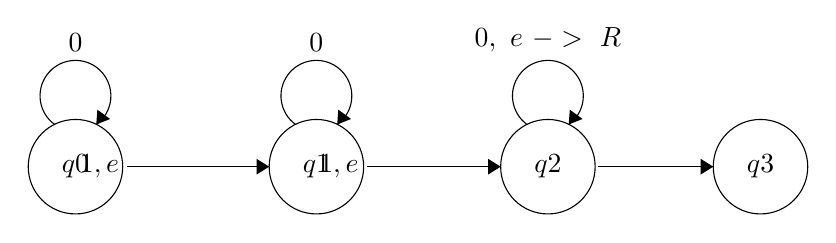
\begin{tikzpicture}[scale=0.2]
	\tikzstyle{every node}+=[inner sep=0pt]
	\draw [black] (16,-30.8) circle (3);
	\draw (16,-30.8) node {$q0$};
	\draw [black] (31.3,-30.8) circle (3);
	\draw (31.3,-30.8) node {$q1$};
	\draw [black] (46,-30.8) circle (3);
	\draw (46,-30.8) node {$q2$};
	\draw [black] (59.5,-30.8) circle (3);
	\draw (59.5,-30.8) node {$q3$};
	\draw [black] (14.677,-28.12) arc (234:-54:2.25);
	\draw (16,-23.55) node [above] {$0$};
	\fill [black] (17.32,-28.12) -- (18.2,-27.77) -- (17.39,-27.18);
	\draw [black] (29.977,-28.12) arc (234:-54:2.25);
	\draw (31.3,-23.55) node [above] {$0$};
	\fill [black] (32.62,-28.12) -- (33.5,-27.77) -- (32.69,-27.18);
	\draw [black] (44.677,-28.12) arc (234:-54:2.25);
	\draw (46,-23.55) node [above] {$0,\mbox{ }e\mbox{ }->\mbox{ }R$};
	\fill [black] (47.32,-28.12) -- (48.2,-27.77) -- (47.39,-27.18);
	\draw [black] (49.2,-30.8) -- (56.5,-30.8);
	\fill [black] (56.5,-30.8) -- (55.7,-30.3) -- (55.7,-31.3);
	\draw [black] (19.3,-30.8) -- (28.3,-30.8);
	\draw (18.8,-30.8) node [left] {$1,e$};
	\fill [black] (28.3,-30.8) -- (27.5,-30.3) -- (27.5,-31.3);
	\draw [black] (34.5,-30.8) -- (43,-30.8);
	\draw (34,-30.8) node [left] {$1,e$};
	\fill [black] (43,-30.8) -- (42.2,-30.3) -- (42.2,-31.3);
	\end{tikzpicture}
\end{center}


%*********************************************************************************
% 2.6 here

%*********************************************************************************
% 2.10 here

%*********************************************************************************
% 2.11 here

%*********************************************************************************
% 2.12 here

%*********************************************************************************
% 2.13 here

%*********************************************************************************
% 2.14 here

%*********************************************************************************
% 2.26 here

%*********************************************************************************
% 2.30 here

%*********************************************************************************
% 2.31 here

%*********************************************************************************
% 2.32 here

%*********************************************************************************
% 2.47 here

\end{document}
